\documentclass{beamer}
\usepackage[utf8]{inputenc}
\usepackage{graphicx}
\usepackage{hyperref}

\usetheme{Madrid}
\usecolortheme{seahorse}

\title{Interaktivni Pong}
\author{Justin Raišp}
\date{10.12.2024}

\begin{document}

\frame{\titlepage}

\begin{frame}
\frametitle{Opis projekta}
\begin{itemize}
    \item Interaktivna različica klasične igre Pong,
    \item uporablja zaznavanje položajev rok za upravljanje loparjev,
    \item implementacija v Pythonu s knjižnico \texttt{pygame},
    \item poudarek na interakciji z uporabo videja in zvoka.
\end{itemize}
\end{frame}

\begin{frame}
\frametitle{Cilji projekta}
\begin{itemize}
    \item Implementacija osnove igre Pong s knjižnico \texttt{pygame},
    \item integracija zaznavanja rok za upravljanje loparjev,
    \item zagotoviti tekoče in naravno gibanje loparjev,
    \item implementacija sistema za štetje točk in prikaz rezultatov,
    \item uporaba zvoka za dodatne funkcionalnosti,
    \item igro predstaviti preko spletne strani.
\end{itemize}
\end{frame}

\begin{frame}
\frametitle{Kaj je že narejeno?}
\begin{itemize}
    \item Osnovna igra Pong (žoga, loparji, točkovanje),
    \item zaznavanje položajev rok z uporabo kamere,
    \item glajenje gibanja loparjev in kazalnikov (rdeč in moder krog),
    \item sistem za štetje točk in prikaz rezultatov,
    \item vizualni prikaz trenutnega stanja igre.
\end{itemize}
\vspace{5mm}
\centering
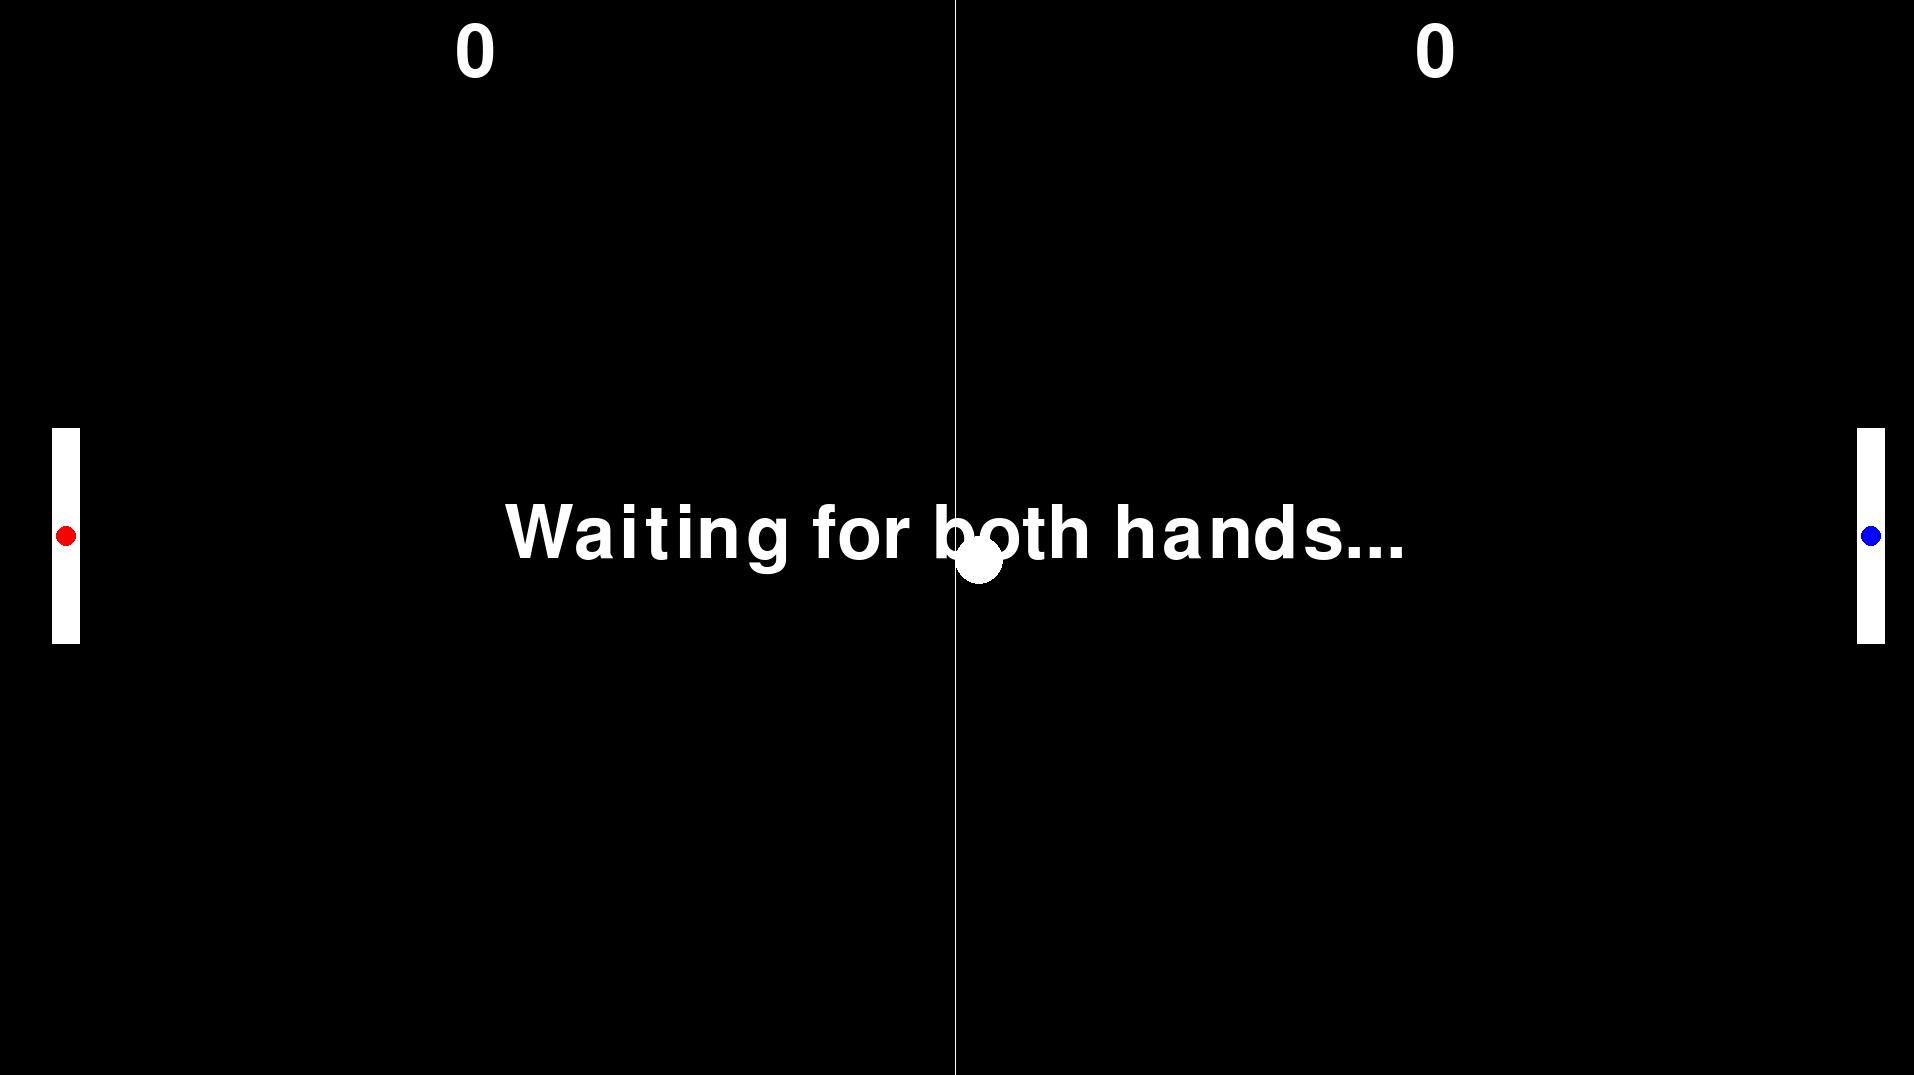
\includegraphics[width=0.7\textwidth]{prototip.png}
\end{frame}

\begin{frame}
\frametitle{Kaj je še treba narediti?}
\begin{itemize}
    \item Optimizacija zaznavanja rok za boljšo odzivnost,
    \item dodajanje zvočnih učinkov in dodatnih funkcionalnosti v sami igri,
    \item izboljšava uporabniškega vmesnika,
    \item spletno stran z igro.
\end{itemize}
\end{frame}

\end{document}
